%----------------------------------------------------------------------------
\chapter{Első fázis}\label{sect:FirstPhase}
%----------------------------------------------------------------------------
\section{Szöveges UseCase(k)}
\subsection{Main Scenerio}
\begin{enumerate}
	\item Jegyzőkönyv kiválasztása.
		\begin{itemize}
			\item Elsődleges aktor: vizsgálatot végző munkatárs
			\item Elsődleges, sikeres forgatókönyv: A vizsgálatot végző munkatárs kiválasztja az alkoholszondás vizsgálat jegyzőkönyv sablont.
		\end{itemize}
	\item A rendszer elküldi a megfelelő sablont.	
	\item Jegyzőkönyv felvétele.
		\begin{itemize}
			\item Elsődleges aktor: vizsgálatot végző munkatárs
			\item Elsődleges, sikeres forgatókönyv: A vizsgálatot végző munkatárs felveszi a vizsgált munkatárs nevét és azonosítóját, illetve a vizsgálatot kérő felettes nevét és azonosítóját, illetve meg kell adnia még a saját nevét és azonosítóját. Ezután a szondás vizsgálat eredménye mellett még megjegyzést is írhat a jegyzőkönyvbe. 
		\end{itemize}
	\item Jegyzőkönyv aláírása.
	\begin{itemize}
		\item Elsődleges aktor: az eljárásban résztvevő személy 
		\item Elsődleges, sikeres forgatókönyv: Az eljárásban résztvevő személy aláírja a jegyzőkönyvet.
	\end{itemize}
	\item A rendszer megerősíti a kitöltött adatok hitelességét.
	\item A rendszer elmenti a jegyzőkönyvhöz tartozó adatokat.
	\item A rendszer üzenetet küld, a sikeres jegyzőkönyv felvételről.
\end{enumerate}

\subsection{Extensions}
\begin{itemize}
	\item Vérvizsgálat opcionális igénylése.
		\begin{itemize}
			\item Elsődleges aktor: vizsgálatot végző munkatárs
			\item Alternatív forgatókönyv: Abban az eseten ha a szondás vizsgálat eredményével nem ért egyet a vizsgált munkatárs, vérvizsgálatot kér. 4-es UseCase következik ez után.
		\end{itemize}
	\item Vérvizsgálati eredmény csatolása.
		\begin{itemize}
			\item Elsődleges aktor: üzemorvos
			\item Alternatív forgatókönyv:  Az üzemorvos tetszőleges jegyzőkönyvhöz mellékletet is csatolhat, természetesen ennek csak akkor van értelme ha a vizsgált munkatárs vérvizsgálatot kér. Minden esetben amikor csatol az üzemorvos valamit egy jegyzőkönyvhöz alá is kell írnia azt, így a 4-es UseCase következik.
		\end{itemize}
	\item \textbf{2/a.} A rendszer elutasítja a jegyzőkönyv sablon kérést a megfelelő jogosultság hiányára hivatkozva. A folyamat a UseCase 1-es lépésétől folytatodik.
	\item \textbf{5/a.} A rendszer hibát talált adatok kitöltésénél. A nem megfelelően kitöltött, vagy érvénytelen adatok mezője mellé piros felkiáltó jelet helyez. 3-as UseCase következik.
	\item \textbf{5/b.} A rendszer hibát talált a fájl csatolásánál. 4-es UseCase következik.
\end{itemize}

\newpage
\section{Aktivitás diagram}

\begin{figure}[!h]
	\centering
	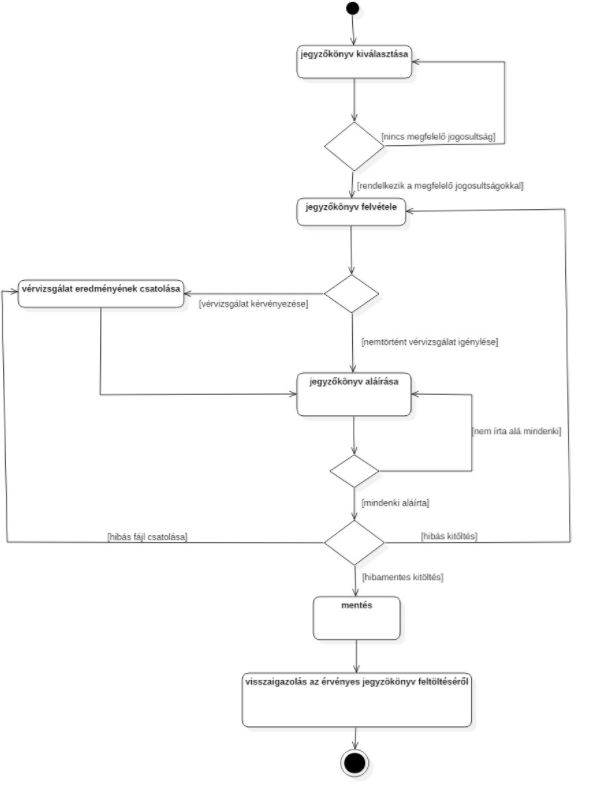
\includegraphics[width=100mm, keepaspectratio]{figures/aktivitas.jpg}
	%\caption{Az aktivitás diagram} 
	%\label{fig:SpiFig}
\end{figure}
\newpage
\section{System sequence diagram}

\begin{figure}[!h]
	\centering
	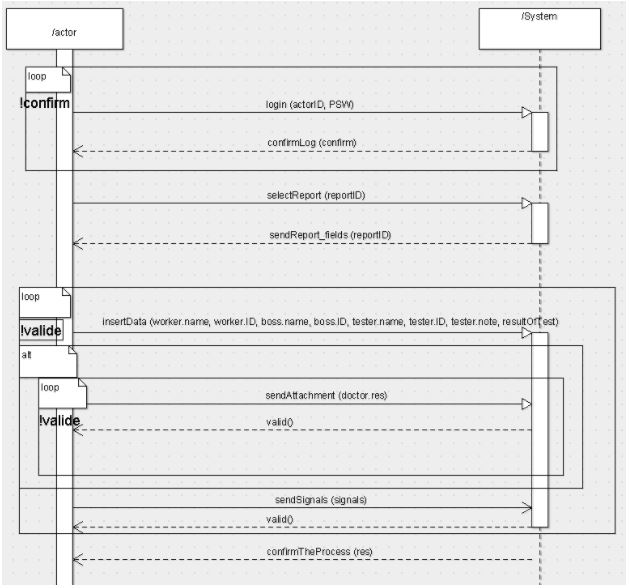
\includegraphics[width=100mm, keepaspectratio]{figures/ssd1.jpg}
	%\caption{Az aktivitás diagram} 
	%\label{fig:SpiFig}
\end{figure}

\begin{figure}[!h]
\centering
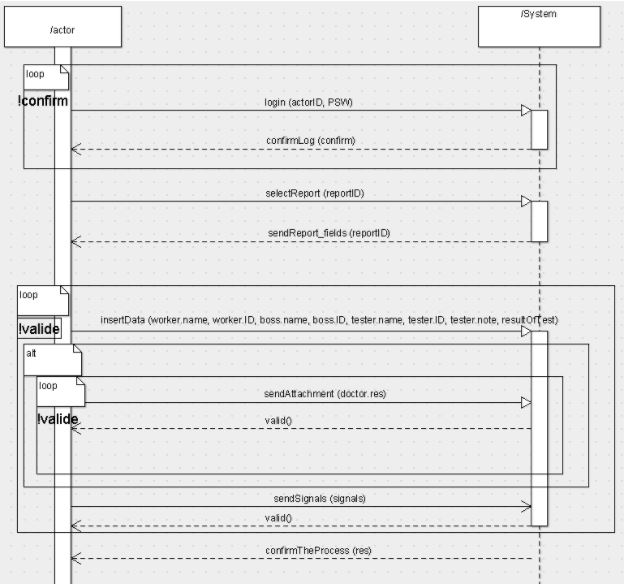
\includegraphics[width=100mm, keepaspectratio]{figures/ssd2.jpg}
%\caption{Az aktivitás diagram} 
%\label{fig:SpiFig}
\end{figure}
